\chapter{Theoretical Background}
\label{chap:Theory}

The theories and discoveries of thousands of physicists since the 1930s have resulted in a remarkable insight into the fundamental structure of matter: everything in the universe is found to be made from a few basic building blocks called fundamental particles, governed by four fundamental forces. Our best understanding of how these particles and three of the forces are related to each other is encapsulated in the Standard Model of particle physics. Developed in the early 1970s, it has successfully explained almost all experimental results and precisely predicted a wide variety of phenomena. Over time and through many experiments, the Standard Model has become established as a well-tested physics theory.



The increasing knowledge about subatomic structures and new particles was accom-
panied by the evolution of quantum mechanics and special relativity. The discovery
of new particles and phenomena required new and adapted theories. Similarly, theor-
etical predictions could be confirmed or excluded by the experiment. This interplay
between theoretical predictions and experimental discoveries lead to a theoretical
description of particle physics that is now called the Standard Model of particle
physics.

\section{Standard Model}
The Standard Model of particle physics describes quarks (q) and leptons as fundamental
constituents of matter. They can be interpreted as structureless fermions, involving parti-
cles with spin 2 1 . Their dynamics is completely determined by a small set of fundamental
interactions, from which - at least in principle - all other laws of physics can be derived.
In the SM, three fundamental interactions are described: the electromagnetic, the weak,
\begin{figure}[!h]
\begin{center}
\vspace*{3mm} 
\hspace*{-5mm}
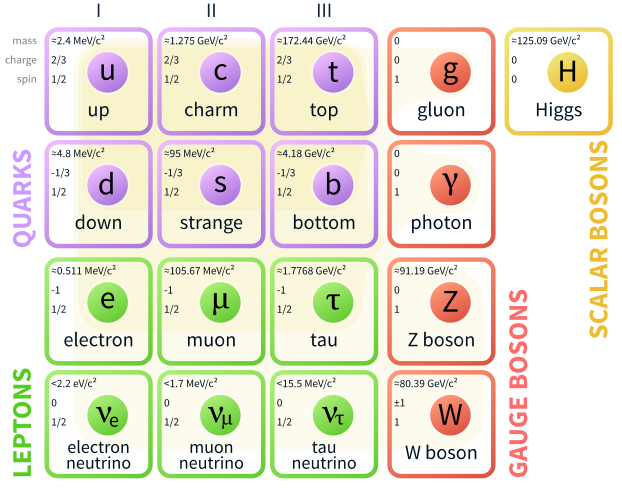
\includegraphics[scale = 0.8]{/home/anter/Desktop/Thesis/Figures/StandardModel_edited.png}\\
\vspace*{4mm}
\caption[Muon]{The Standard Model of elementary particles, with the three generations of matter, gauge bosons in the fourth column, and the Higgs boson in the fifth column\footnotemark.}
\label{fig:muon}
\end{center}
\end{figure}
\footnotetext{Source : \url{https://en.wikipedia.org/wiki/Standard_Model}}

\section{Quantum Chromodynamics}
\subsection{Perturbative Quantum Chromodynamics}
\subsection{The Strong Coupling Constant}
\subsection{Parton Density Functions}

\section{Hadron Collisions}
\subsection{Parton Shower}
\subsection{Hadronization}
\subsection{Underlying Event and Multi-Parton Interactions}

\section{Jets}
\label{sec:jets}
\subsection{Jet Algorithms}
\label{sec:jet_algos}

\subsection{Jet Properties}

\cleardoublepage

\begin{comment}
\section{The Standard Model}
The theories and discoveries carried out by physicists over a long time have resulted in revealing the fundamental structure of matter. The matter of the Universe is made up of twelve building blocks which are called fundamental particles, governed by the four fundamental forces ~\cite{Griffiths}. The present knowledge of these fundamental particles and their relation with the forces is summarized in the Standard Model ~\cite{stand,stand1} of particles and forces.

According to the Standard Model, all matter is made up of three kinds of fundamental particles : $quarks$ (must bind together), $leptons$ (can exit independently) and $mediators$. The quarks and leptons, known as partons, are the building blocks and the mediators mediate the forces between them. Quarks and leptons are fermions having half integral spin and mediators are gauge bosons having spin either 0 or integral. These have no internal structure and hence are called fundamental particles. 

There are six types of leptons : electron ($e^-$), muon ($\mu^-$) and tau ($\tau^-$) with  electric charge Q = $-1$ (all charges are in the units of elementary charge $e$) and the corresponding neutrions $\nu_e$, $\nu_\mu$ and $\nu_\tau$ having  electric charge Q = 0. 

The quarks carry fractional charges $\pm$ $\frac{2}{3}$, $\pm$ $\frac{1}{3}$. There are six ``flavors'' of quarks : $up$, $down$, $strange$, $charmed$, $bottom$ and $top$. Each quark and lepton has an anti-quark and an anti-lepton, respectively with same mass but an opposite charge.
The quarks and leptons are classified into three generations as shoen in Table \ref{gen}:


\begin{table}[ht]
\begin{center}
\begin{tabular}{|c|c|c|}
\hline
& Quarks   &   Leptons \\

\hline

 Generation-I    &  up (u)       &   electron (e) \\
                 &  down (d)     &   e-neutrino ($\nu_e$)\\
\hline
 Generation-II   &  charm (c)    &   muon ($\mu$)\\
                 &  strange (s)  &   $\mu $-neutrino ($\nu_\mu$)\\
\hline
 Generation-III  &  top (t)      &   tau ($\tau $) \\   
                 &  bottom (b)   &   $\tau $-neutrino ($\nu_\tau$) \\
\hline
          
\end{tabular}
\caption{Generations of quarks and leptons.}
\label{gen}
\end{center}
\end{table} 

The lightest and the most stable particles belong to first generation and the second and third generations have the heavier and less stable particles.

There are four kinds of fundamental forces : the  gravitational force, the weak force, the electromagnetic force and the strong force. These forces have different strengths and ranges. The gravity is the weakest and has an infinite range. The weak and strong forces are effective over a small range. The electromagnetic force is stronger than the gravity but has an infinite range. Every interaction involves the exchange of a gauge boson : the photon for the electomagnetic force, two W's and a Z for the weak force, the graviton (not yet found) for the gravitational force and 8 gluons for the strong force. Gluons are responsible for binding the quarks. 

\section{Quantum Chromodynamics}
Quantum Chromodynamics ~\cite{qcd1,qcd2} is the theory to describe the strong interaction between the quarks. The strong force is mediated through the exchange of gluons. Both the quarks and gluons carry a type of charge called ``color'' charge which is conserved. There are three different color charges and anti-color charges. The colors are usually red, green and blue. As quarks carry a single color charge so come in three varieties of color but as gluons carry a combination of color charges so come in eight combinations. Hadrons are strongly interacting colorless particles made up of two types of quark combination : $baryons$ (three quarks) and $mesons$ (quark-antiquark pair). QCD has two properties:

\subsection{Confinement}
Although the quarks and gluons themselves carry color charge, the hadrons are always neutral in color. The quarks are never observed as free entities. When the colored quarks and gluons within the hadron are pulled farther and farther apart, there is an increase in the strength of force between them. This results in creation of new quark-antiquark pair making diificult to liberate a free quark or gluon. This property is known as ``confinement'' ~\cite{con,con1}. As it would take an infinite amount of energy to seperate two quarks, they are forever bound into hadrons as the proton and the neutron. So far, no one has provided a conclusive proof for QCD confinement.
     
\subsection{Asymptotic freedom}
The strength of the interaction is given by a fundamental parameter called the coupling constant. In QED, the coupling constant ($\alpha$) is constant. In contrast to this, in QCD, the coupling constant ($\alpha_s$) is not constant and depends on the seperation between the interacting particles. It increases with the increase in the distance. So at higher energies or smaller distances, the quarks and gluons interact very weakly. This is the property of ``asymptotic freedom'' of quarks.    

\section{Jet Production}
The high-energy phenomenon involving quantum chromodynamics (QCD) is discussed commonly  in terms of quarks and gluons. The property of confinement is responsible for the production of jets in high energy collisions of hadrons. According to the Heisenberg uncertainity principle, the beams with high momentum probe the small distance within the  hadron. At high energy, a single parton gets probed within each incoming hadron. So the collision between two hadrons is visualised as a collision between two quarks or two gluons or a quark and a gluon. A quark or a gluon is never visible as after the collision, it begins to get separated from the rest of partons. With the increase in distance, the strength of the force of interaction increases and there is enough energy to create a particle-antiparticle pair. This process continues which leads to the formation of the stable hadrons collimated in the form of bunches. This results in the formation of the jets - spray of hadronic particles. Jets are the final structures observed in the detector. By measuring their energy and direction, we can get close to the original ``parton''. The jet definitions or algorithms are needed to precisely define the jets. The evolution of a jet is illustrated in Figure \ref{ev_j}. A parton that has not yet undergone fragmentation is sometimes referred to as a parton level jet.
A moving parton will radiate gluons and create quark-antiquark pairs by fragmentation and the resulting spray of partons is usually referred to as a parton cascade. The coloured particles within such a cascade
are combined into colourless hadrons through a process called hadronization. The shower
of produced hadrons is usually referred to as a particle level jet.
A jet reconstructed from the energy deposited in a calorimeter by a
particle level jet is referred to as a calorimeter level jet.

\begin{figure}[h!]
\begin{center} 
\includegraphics[scale = 0.75]{figs/Theoretical/jet.pdf}
\caption{Evolution of a jet.}
\label{ev_j}
\end{center}
\end{figure} 
 
\section{Jet Algorithms}
Jet algorithms provide a set of rules for grouping the particles into jets. They usually involve one or more parameters that indicate how close two particles must be for them to belong to the same jet. They can either measure closeness in coordinate space (cone algorithms) or in momentum space (sequential algorithms). They should be able to operate on parton, particle and calorimeter levels. They are always associated with a recombination scheme, to indicate what momentum is assigned to the combined particles. A jet algorithm with its parameters and a recombination scheme forms a ``jet definition''. 
Several important properties that should be met by a jet definition are ~\cite{S.D.} :\\
1. Simple to implement in an experimental analysis;\\
2. Simple to implement in the theoretical calculation;\\
3. Defined at any order of perturbation theory;\\
4. Yields finite cross section at any order of perturbation theory;\\
5. Yields a  cross section that is relatively intensive to hadronization.\\

The basic jet kinematics is as following :
The coordinate system is shown in Figure \ref{coordsysI} where r is the radial distance, $\phi$ is the azimuthal angle such that $\phi$ = 0 points to the +x-axis and $\phi$ = $\pi$/2 to the y-axis, and $\theta$ is the polar angle such that $\theta$ = 0 corresponds to +z-axis and $\theta$ = $\pi$ to the -z-axis.

\begin{figure}[h!]
\begin{center} 
\includegraphics[scale = 0.75]{figs/Theoretical/coordinate.jpeg} 
\caption{The coordinate system showing the polar angle ($\theta$), radial
distance (r) and azimuthal angle ($\phi$).}
\label{coordsysI}
\end{center}
\end{figure}  

For a fixed particle mass, a relativistically invariant phase space volume d$\tau$ for a particle of momentum $\vec {p}$ and energy E is given by
\begin{equation}
d\tau = \frac  {d^3p}{E} = \frac {dp_xdp_ydp_z}{E}
\end{equation} 
Taking z as the collision axis, neither E nor $p_{z}$ are invariant Lorentz transformation. The variables for a suitable choice for analysis is ($P_{T},y,\phi,m$) where $P_{T}$ is transverse momentum to $\hat{z}$ direction, $\phi$ is azimuthal angle about  $\hat{z}$, m is mass and $\emph{y}$ is rapidity defined as :
\begin{equation}
y = \frac{1}{2}ln\frac{(E + p_z)}{(E - p_z)}
\end{equation}
For particles with p $\gg$ m = $\sqrt{E^2 - p^2}$,\\
\begin{equation}
y \approx  -ln(tan(\theta /2)) \equiv \eta
\end{equation}
where $\eta$ is pseudo-rapidity.\\
P$_{T}$ is always defined in terms of the 3-momentum $\vec{p}$ as 
\begin{equation}
P_{T} = \bf {p}\sin\theta
\end{equation}
The transverse energy $E_{T}$ is given by
 \begin{equation}
E = E_{T}\cosh y
\end{equation}
or
 \begin{equation}
p_z = E_{T}\sinh y
\end{equation}
where 
\begin{equation}
p_z = E\tanh y
\end{equation}

The kinematic properties of the jets (P$_{T}$,$\eta$,$\phi$) can be associated to that of the original partons produced and these are directly measureable.


\subsection{Collinear safety}
Collinear safety is the property by virtue of which the set of hard jets found in the event should not be changed on modification of the event by a collinear splitting i.e. replacement of  one parton by two at the same place. An algorithm should be collinear safe. The output of the jet algorithm remains the same if the energy of a particle is distributed among two collinear particles and the collinear singularities should not appear in the perturbative calculations. Two pictures shown in Figure \ref{coll}
 should  always produce a single jet. Algorithms which produce zero or two jets (in case of left picture)
are not collinear safe. 
 
\begin{figure}[h!]
\begin{center} 
\includegraphics[scale = 0.55]{figs/Theoretical/collinear_safe.png}
\caption{An example of collinear unsafe behavior of jet algorithm is shown. The right
picture shows the situation if the algorithm constructs one jet. In the left picture due to radiation effect if one jet splits up into two parts. In this worst case no jet
would be produced by seeded algorithm, as both small jets would fall below the threshold.}
\label{coll}
\end{center}
\end{figure}

\subsection{Infrared safety}
Infrared safety is the property due to which the addition of a soft emission i.e. addition of a soft gluon should not change or modify the set of hard jets found in the event. The algorithm should be infrared safe. Along with this, it should also find solutions which are insensitive to soft radiation in the event. The algorithms which look for jets around seeds only can be sensitive to soft radiation as shown in Figure \ref{infra1}. With a soft
gluon emission in the middle of two cone jets, this could lead to overlap
of the two initial cones.
 
\begin{figure}[h!]
\begin{center} 
\includegraphics[scale = 0.55]{figs/Theoretical/infrared_safe.png}
\caption{ Infrared unsafe behavior of jet algorithm is illustrated that how the presence of soft radiation between two jets may cause a merging of the jets that would not occur in the absence of the soft radiation.}
\label{infra1}
\end{center}
\end{figure} 


The motivation behind constructing the jets is to view the events in a way which is insensitive to these effects. The details of various algorithms is given below.

\subsection{Cone algorithms}
In the cone algorithm ~\cite{RunII}, the jet is defined as a cone with fixed radius in $\eta-\phi$ space drawn around the highest energy seed. The set of initial particles over a P$_{T}$ threshold or the midpoints between the previous stable cones can be taken as seeds. The jets are defined as dominant directions of energy flow. The algorithm iterates until the cone is stable which means that the direction of sum of momentum of all the particles is same as that of the center of cone. If we consider the 3-particle event as shown in Figure \ref{infra} and clustering is done using midpoint cone algorithm, 2 stable cones are found leading to 2 jets, shown in (a). If a soft gluon is added to this hard event as shown in figure(b), a third stable cone is found. This change the jet structure on addition of a soft particle and makes the algorithm infrarde unsafe. This algorithm is also not collinear safe. 

\begin{figure}[h!]
\begin{center} 
\includegraphics[scale = 1.10]{figs/Theoretical/infraf.png}
\caption{ Stable cones found by the midpoint algorithm for a 3-particle event (left) and for
the same event with an additional infinitely soft gluon (right).}
\label{infra}
\end{center}
\end{figure} 

\subsection{Seedless Infrared-Safe cone (SIS-Cone) algorithm}
The Seedless Infrared-Safe cone (SIS-Cone) algorithm ~\cite{Sis} is an exact seedless cone algorithm that probably identifies all stable cones. It does not rely on seed threshold and it is infrared and collinear safe. This is a complex approach which tests the stability of all subsets of particles and has a complexity of order N$2^{N}$ for N particles, much slower than that of order $N^{3}$ of the midpoint algorithm thus making it unusable for experimental purposes. But this can be reduced to order of $N^{2}$logN ~\cite{Sis} thus making it faster than the midpoint algorithm. 

\subsection{Sequential algorithms}
The sequential algorithm works by defining a distance between pairs of particles and recombining the pair of closest particles successively. This algorithm stops when all the resulting objects are far apart. This is collinear and infrared safe algorithm. It is 
possible for jet cones to overlap such that one particle is contained in more than one jet but the sequential algorithm never 
assigns a particle to more than one jet. The algorithms belonging to this class are:

\subsubsection{$k_{T}$ -algorithm}
The longitudinally invariant $k_{T}$ jet finder ~\cite{Kt1,Kt2} is the most widely used clustering jet finder for proton-(anti)proton collisions. It allows a well defined comparison to the theoretical predictions. 
By restricting ourselves to the approximation that particles are massless, we will have a look at the kinematic variables used 
to represent particle momenta and distances between them. A particle momentum vector {k}, in polar coordinates can be represented as,
\begin{equation}
\vec{k} = (k_{x},k_{y},k_{z}) = \frac {E}{c} \times (\sin\theta\cos\phi,\sin\theta\sin\phi, \cos\theta), 
\end{equation}

where E denotes the particle's energy and taking the incoming particles along the $\pm$z direction.\\
The kinematic properties : transverse momentum $k_{t}$ = $\sqrt{k_{x}^{2} + k_{y}^{2}}$ and the azimuthal angle $\phi$ are longitudinally 
invariant whereas the polar angle trasforms in a complicated manner so a quantity called pseudo-rapidity is used,\\
\begin{equation}
\eta =  -ln(tan(\theta/2)) 
\end{equation}
In the $k_{T}$ jet finder, the distance measure is 
\begin{equation}
d_{ij} = min(k_{t,i}^{2},k_{t,j}^{2}) \frac{\Delta R_{ij}^{2}}{R^{2}},  \hspace{2 cm}   \Delta R_{ij}^{2} = (\eta_i -\eta_j)^{2} +  (\phi_i -\phi_j)^{2},
\end{equation}
where $k_{t,i}, \eta_i,\phi_i$ are the transverse momentum, pseudo-rapidity and azimuthal angle of particle i and R is jet-radius parameter,\\
and  the particle-beam distance is 
\begin{equation}
d_{iB} = k_{t,i}^{2}.
\end{equation}

Procedure for clustering the particles into jets is as follows:
\begin{itemize}
\item
 Calculate the distance $d_{ij}$ for each pair of particles i and j and distance $d_{iB}$ for each parton i.
\item 
Find the minimum  $d_{min}$ of all the $d_{ij},d_{iB}$.
\item
 If $d_{min}$ is  $d_{ij}$ then merge the particles i and j into a new single particle k ,summing their ``four-momenta'' by recombination scheme and go to step 1. 
\item
 If $d_{min}$ is  $d_{iB}$ , declare particle i to be a final-state jet and remove it from the list. 
\item 
Go to step 1.\\
\end{itemize}

The procedure continues until no particles are left. This is an inclusive mode of clustering. In an  exclusive mode of clustering,
 the difference is that the clustering is terminated when all  $d_{ij}$,$d_{iB}$ are above the quantity $d_{cut}$ given by $d_{cut} = y_\mathrm{cut}p_{T}^{2}$(jet), where $y_\mathrm{cut}$ is the dimensionless resolution parameter.


\subsubsection{Cambridge/Aachen algorithm}
The formulation of the Cambridge/Aachen algorithm ~\cite{Camb} is similar to that of 
the $k_{T}$ jet algorithm with the difference that the inter-particle distance measure is 

\begin{equation}
d_{ij} = \frac{\Delta R_{ij}^{2}}{R^{2}},  \hspace{2 cm}   \Delta R_{ij}^{2} = (\eta_i -\eta_j)^{2} +  (\phi_i -\phi_j)^{2},
\end{equation}

and the particle-beam distance is 
\begin{equation}
d_{iB} = 1.
\end{equation}

To extract the jets from the Cambridge/Aachen algorithm exclusively with a $d_{cut}$ parameter, the clustering 
continues up to point where all $d_{ij},d_{iB} > d_{cut}$.

The distance measures can be generalised for the algorithms as : 

\begin{equation}
d_{ij} = min(k_{t,i}^{2p},k_{t,j}^{2p}) \frac{\Delta R_{ij}^{2}}{R^{2}},  \hspace{2 cm}   \Delta R_{ij}^{2} = (\eta_i -\eta_j)^{2} +  (\phi_i -\phi_j)^{2},
\end{equation}
\begin{equation}
d_{iB} = k_{t,i}^{2p}
\end{equation}

where parameter $\emph{p}$ = 1 for the  $k_{T}$ algorithm, 0 for  the Cambridge/Aachen algorithm and -1 for the 
anti-$k_{T}$ algorithm ~\cite{AntiKt}. These algorithms are included in the FastJet Package ~\cite{FastJet,FastJet1,FastJet2}, which is used to cluster the particles into jets in a much faster way. The clustering by $k_{T}$ algorithm involves soft particles and that by anti-$k_{T}$ algorithm involves hard particles whereas the Cambridge/Aachen algorithm involves energy independent clusterings. In the anti-$k_{T}$ algorithm, a collinear branching gets clustered at the beginning of the sequence making it collinear and infra-red safe and thus a good substitute for the cone-type algorithms. The $k_{T}$ and the Cambridge/Aachen algorithms give irregular jets but the anti-$k_{T}$ algorithm gives circular hard jets.

\subsection{Recombination Schemes}
A jet algorithm must specify how to combine different partons or particles into a single four-vector. The most widely used recombination scheme is the E-scheme ~\cite{RunII}, or 4-vector recombination scheme which simply adds the four vectors. This has been given as a standard in ~\cite{RunII}. This was the main scheme in use during RUN II of the Tevatron. It is the default option in FastJet ~\cite{FastJet} and is currently used by the LHC experiments. We have also used this in the present work. This scheme calculates the 4-momentum
 of the jet from the 4-momentum of the invidual constituents by adding the four-vectors of merging particles i.e. $E = \sum E^{i}, k_{t,x,y,z} = \sum k_{t,x,y,z}^{i}$ where the summation is over all the particles of the jet.
The various recombination schemes have been used experimentally. They differ in the way in which the resolution variables are defined after two particles have been merged into a single one. The data is insensitive to which scheme is used. 
The different types of recombination schemes are :
\begin{itemize}
\item
E$\_$scheme
\item
pt$\_$scheme
\item
pt2$\_$scheme
\item
Et$\_$scheme
\item
Et2$\_$scheme
\item
BIpt$\_$scheme
\item
BIpt2$\_$scheme
\end{itemize}

The p$_{t}$, p$_{t}^{2}$, E$_{t}$ and E$_{t}^{2}$ schemes involve a preprocessing stage to make the initial momemta massless. In the preprocessing stage, rescaling is done to the energy to be equal to the 3-momentum for the  p$_{t}$ and p$_{t}^{2}$ schemes and rescaling is done to the 3-momentum to be equal to the energy in the  E$_{t}$ and E$_{t}^{2}$ schemes. For all the four schemes, the recombined p$_{r}$ of p$_{i}$ and p$_{j}$ is a massless 4-vector which satisfies 
\begin{equation}
p_{t,r} =  p_{t,i} + p_{t,j}\\
\end{equation}
\begin{equation}
\phi_{r} = (w_{i}\phi_{i} + w_{j}\phi_{j})/(w_{i} + w_{j})\\
\end{equation}
\begin{equation}
y_{r} = (w_{i}y_{i} + w_{j}y_{j})/(w_{i} + w_{j})\\
\end{equation}
where $\emph{w}_{i}$ is $\emph{p}_{t,i}$ for the p$_{t}$ and E$_{t}$ schemes, and is $\emph{p}_{t,i}^{2}$ for the p$_{t}^{2}$ and E$_{t}^{2}$ schemes. $\emph{p}_{t,i}$, $\phi_{i}$, $\emph{y}_{i}$ are the transverse momentum, azimuthal angle and rapidity of particle i respectively.
As these schemes are not longitudinally invariant for the massive particles, BIpt$\_$scheme and BIpt2$\_$scheme are available. They are identical to the normal p$_{t}$ and p$_{t}^{2}$ schemes with the difference that they do not involve the preprocessing stage.

\section{Subjets}
The internal structure of jets provides an insight into the transition between partons produced in the hard scattering process and the experimentally observable jets of hadrons. The substructure of jets is expected to mainly depend on the type of primary parton, quark or gluon, and the particular hard scattering process but to a lesser extent. The substructure of jets can be studied in terms of the integrated jet shape, $\psi$(r),and the differential jet shape, $\rho$(r), where the energy flow inside a jet is considered, and the subjet multiplicity, <${n_{subj}}$>, where subjets (jet-like structures) within a given jet are studied. The subjets in a particular jet are defined by re-running the jet algorithm only on the particles assigned to a jet .

Unlike for the $k_{T}$ and the Cambridge/Aachen algorithms, 
the anti-$k_{T}$ recombination sequence will slowly expand through a soft subjet, rather than first constructing the soft subjet and then recombining it with a hard subjet. The anti-k$_{T}$ jet algorithm is also a sequential recombination algorithm which merges the particles with high relative P$_{T}$ into jets. So the soft particles within the size R of a high P$_{T}$ jet will be merged with it. So it is less senstive to details of the distribution of softer objects in an event (or within jets) as it starts clustering with the hardest (highest p$_{T}$) objects in an event. Hence it is less well suited for an investigation of jet substructure. So the clustering sequence inside an anti-$k_{T}$ jet is not usefully related to QCD 
branching.

With k$_{T}$ algorithm, the clustering of the particles in a jet is terminated when all  $d_{ij}$,$d_{iB}$ are above the quantity $d_{cut}$ given by $d_{cut} = y_\mathrm{cut}p_{T}^{2}$(jet) ~\cite{dcut}, where $y_\mathrm{cut}$ is the dimensionless resolution parameter such that  0$\leq y_\mathrm{cut} \leq$1 and $p_{T}$(jet) is the transverse momentum of the jet. The parameter $y_\mathrm{cut}$ defines the minimal relative transverse energy between subjets inside the jet and thus determines the extent upto which the internal jet structure can be resolved. 
In Cambridge/Aachen algorithm, after clustering with some given value of R, the constituents of a particular jet can be clustered into subjets by re-running the algorithm at a smaller radius, $R_{eff}$ = $\sqrt{d_{cut}}$R.

\subsection{Subjet Multiplicity}
The subjet multiplicity is a natural observable of the k$_{T}$ algorithm. The number of subjets in a jet is the subjet multiplicity M. In the computer implementation, for any value of $y_\mathrm{cut}$, the subjets can be reconstructed in a fast way as the algorithm keeps a record of all the vectors merged into a jet. For $y_\mathrm{cut}$ = 1, M =1 i.e. every jet consists of a single subjet while for $y_\mathrm{cut} \rightarrow $0, every particle in the jet is a subjet. With the decrease in $y_\mathrm{cut}$, the subjet multiplicity increases. Two subjets are resolved within a jet if they are non-collinear means well seperated in $\eta \times \phi$ space or if both are hard i.e. carry a significant fraction of the jet P$_{T}$. In Cambridge algorithm, for Rsub = R, the number of subjets in each jet is one. With the decrease in Rsub, the subjet multiplicity increases.
\section{Ratio of Color factor}
In QCD, the quarks and gluons have different color charges which results in different coupling strengths. The color factors C$_{A}$ and C$_{F}$ having values 3 and 4/3 respectively form the basis of QCD. These values have been derived theoretically from the symmetry group SU(3) of QCD whose details can be seen in ~\cite{qcd2}. C$_{A}$ determines the relative probability for a soft gluon to couple with another gluon and C$_{F}$ determines the corresponding probability for a
soft gluon to couple with a quark. Besides the strong interaction coupling strength, $\alpha_{S}$, the ratio  C$_{A}$/C$_{F}$
is the most fundamental quantity in QCD. As C$_{A}$/C$_{F}$ = 9/4 = 2.25, a gluon is more likely to radiate than a quark. This is because of an increase in color charge of a gluon relative to a quark and the number of subjets emitted in gluon jets is measured to be approximately twice that in quark jets. The various properties of gluon and quark jets in terms of subjet variables can be studied and used to measure the ratio C$_{A}$/C$_{F}$. We have used subjet multiplicity property to find the color factor ratio. The subjet multiplicity M variable is useful in determining the color factor ratio given by
 \begin{equation}
r = \frac{<M_{g}>-1}{<M_{q}>-1}
\end{equation}
such that r = 1 indicates that gluon jets are not different from quarks. Any other value than unity signifies the difference between a quark and a gluon. Here $<M_{g}>$ and $<M_{q}>$ are the average subjet multiplicityies in gluon and quark jets respectively.

Predictions at NLO accuracy in pQCD are computed with the \NLOJETPP
program version~4.1.3~\cite{Nagy:2001fj,Nagy:2003tz}. The results are
provided within the framework of \fastNLO
version~2.3~\cite{Britzger:2012bs} for use within fits. The
renormalization and factorization scales \mur and \muf are chosen
equal to \httwo. PDF sets at NLO available for a series of different
assumptions on \alpsmz via the \LHAPDFS package~\cite{Buckley:2014ana}
are listed in Table~\ref{tab:chap2:nlopdfsets}. All sets employ a
variable-flavour number scheme with at most five or six flavours apart
from the ABM11 PDFs, which use a fixed-flavour number scheme with
$\NF=5$.

Out of these eight PDF sets the following three will not be considered
further:
%
\begin{itemize}
\item At NLO, predictions based on ABM11 do not describe LHC jet data
  at small jet rapidity, cf.\ Refs.~\cite{Aad:2013lpa, Aad:2014vwa,
    CMS:2014mna, Khachatryan:2015luy}.
\item The HERAPDF2.0 set exclusively fits HERA DIS data with only weak
  constraints on the gluon PDF\@.
\item The range in values available for \alpsmz is too limited for the
  NNPDF3.0 set.
\end{itemize}
%

PDF uncertainties are evaluated according to the prescriptions given
for each PDF set. Uncertainties on \alpsmz are not considered, since
this value is later on determined from a fit to the data. The PDF
uncertainty as derived with the CT10 PDF set ranges from 2\% to 30\%
for inclusive 2- and 3-jet cross sections and from 2\% to 7\% for \ratio.

\begin{table}[htbp]
  \centering
  \caption{NLO PDF sets available via \LHAPDFS for comparisons to data with
    various assumptions on the value of \alpsmz. Sets existing already in
    LHC Run~1 (upper rows) and newer sets for Run~2 (lower rows) are
    listed together with the corresponding number of flavours \NF, the
    assumed masses $M_t$ and $M_Z$ of the top quark and the $Z$ boson,
    respectively, the default values of \alpsmz, and the range in \alpsmz
    variation available for fits.  A~$^*$ behind the \alpsmz values
    signifies that the parameter was fixed, not fitted.}
  \label{tab:chap2:nlopdfsets}
  \begin{tabular}{llccllc}
    \hline\hline
    Base set & Refs. & \NF & $M_t$ (\GeVns{}) &
    $M_Z$ (\GeVns{}) &\alpsmz & \alpsmz range\rbthm\\
    \hline
    % LHC Run 1
    ABM11     & \cite{Alekhin:2012ig}
    &       5   & 180       & 91.174  & $0.1180$   & 0.110--0.130\rbtrr\\
    CT10      & \cite{Lai:2010vv}
    & ${\leq}5$ & 172       & 91.188  & $0.1180^*$ & 0.112--0.127\rbtrr\\
    MSTW2008  & \cite{Martin:2009iq,Martin:2009bu}
    & ${\leq}5$ & $10^{10}$ & 91.1876 & $0.1202$   & 0.110--0.130\rbtrr\\
    NNPDF2.3  & \cite{Ball:2012cx}
    & ${\leq}6$ & 175       & 91.1876 & $0.1180^*$ & 0.114--0.124\rbtrr\\\hline
    % LHC Run 2
    CT14      & \cite{Dulat:2015mca}
    & ${\leq}5$ & 172       & 91.1876 & $0.1180^*$ & 0.113--0.123\rbtrr\\
    HERAPDF2.0& \cite{Abramowicz:2015mha}
    & ${\leq}5$ & 173       & 91.1876 & $0.1180^*$ & 0.110--0.130\rbtrr\\
    MMHT2014  & \cite{Harland-Lang:2014zoa}
    & ${\leq}5$ & $10^{10}$ & 91.1876 & $0.1180^*$ & 0.108--0.128\rbtrr\\
    NNPDF3.0  & \cite{Ball:2014uwa}
    & ${\leq}5$ & 173       & 91.2    & $0.1180^*$ & 0.115--0.121\rbtrr\\
    \hline\hline
  \end{tabular}
\end{table}

The uncertainty related to unknown higher orders of the perturbative
series is evaluated with the conventional recipe of varying the
default scale \httwo chosen for \mur and \muf independently in the
following six combinations: (\mur/\httwo, \muf/\httwo) = (1/2,1/2),
(1/2,1), (1,1/2), (1,2), (2,1) and (2,2). The maximal upwards and
downwards deviations in cross section from the central prediction are
taken as scale uncertainty. This uncertainty ranges for inclusive
2-jet events from 5\% to 13\%, for inclusive 3-jet events from 11\%
to 17\% and for their ratio \ratio from 6\% to 8\%.

The computation of the NLO predictions with \NLOJETPP is also subject
to statistical fluctuations from the numerical integrations.  For the
inclusive 2-jet event cross sections this uncertainty is smaller than
about one per mille, while for the inclusive 3-jet event cross section
it amounts to 1--9 per mille.

Higher order effects of electroweak origin affect jet cross sections at large
jet \pt. These electroweak (EWK) corrections have been calculated for
the inclusive 1-jet and 2-jet case, cf.\ Ref.~\cite{Dittmaier:2012kx},
but are not yet known for 3-jet production. Therefore, they are
considered for the 2-jet events, while for the 3-jet event cross
section and for the ratio they have been neglected.

The impact of nonperturbative (NP) effects, \ie from multiple-parton
interactions (MPI) and hadronization, are evaluated by using samples
obtained from different MC event generators with a simulation of
parton-shower and underlying-event (UE) contributions. The leading
order (LO) MC event generators \HERWIGPP~\cite{Bahr:2008pv} with the
default tune of version~2.3 and \PYTHIAS~\cite{Sjostrand:2006za} with
tune \Ztwostar are considered, and the dijet NLO prediction from
\POWHEG~\cite{Nason:2004rx, Frixione:2007vw, Alioli:2010xa} interfaced
to \PYTHIAE with tune CUETS1~\cite{Khachatryan:2015pea} for full event
generation. The cross section ratios between a nominal event
generation and a sample without hadronization and MPI effects are
taken as correction separately for inclusive 2-, and 3-jet events, and
as their ratio for \ratio. This ratio is fitted by a power-law
function. The differences in the correction factors obtained from the
various MC event generators are assigned as an uncertainty. The
central correction factors $C^{\mathrm{\tiny{NP}}}$ are determined by
the centre of the envelope which covers all predictions and half of
the spread is taken as the uncertainty.

\begin{figure}[h]
  \hftwo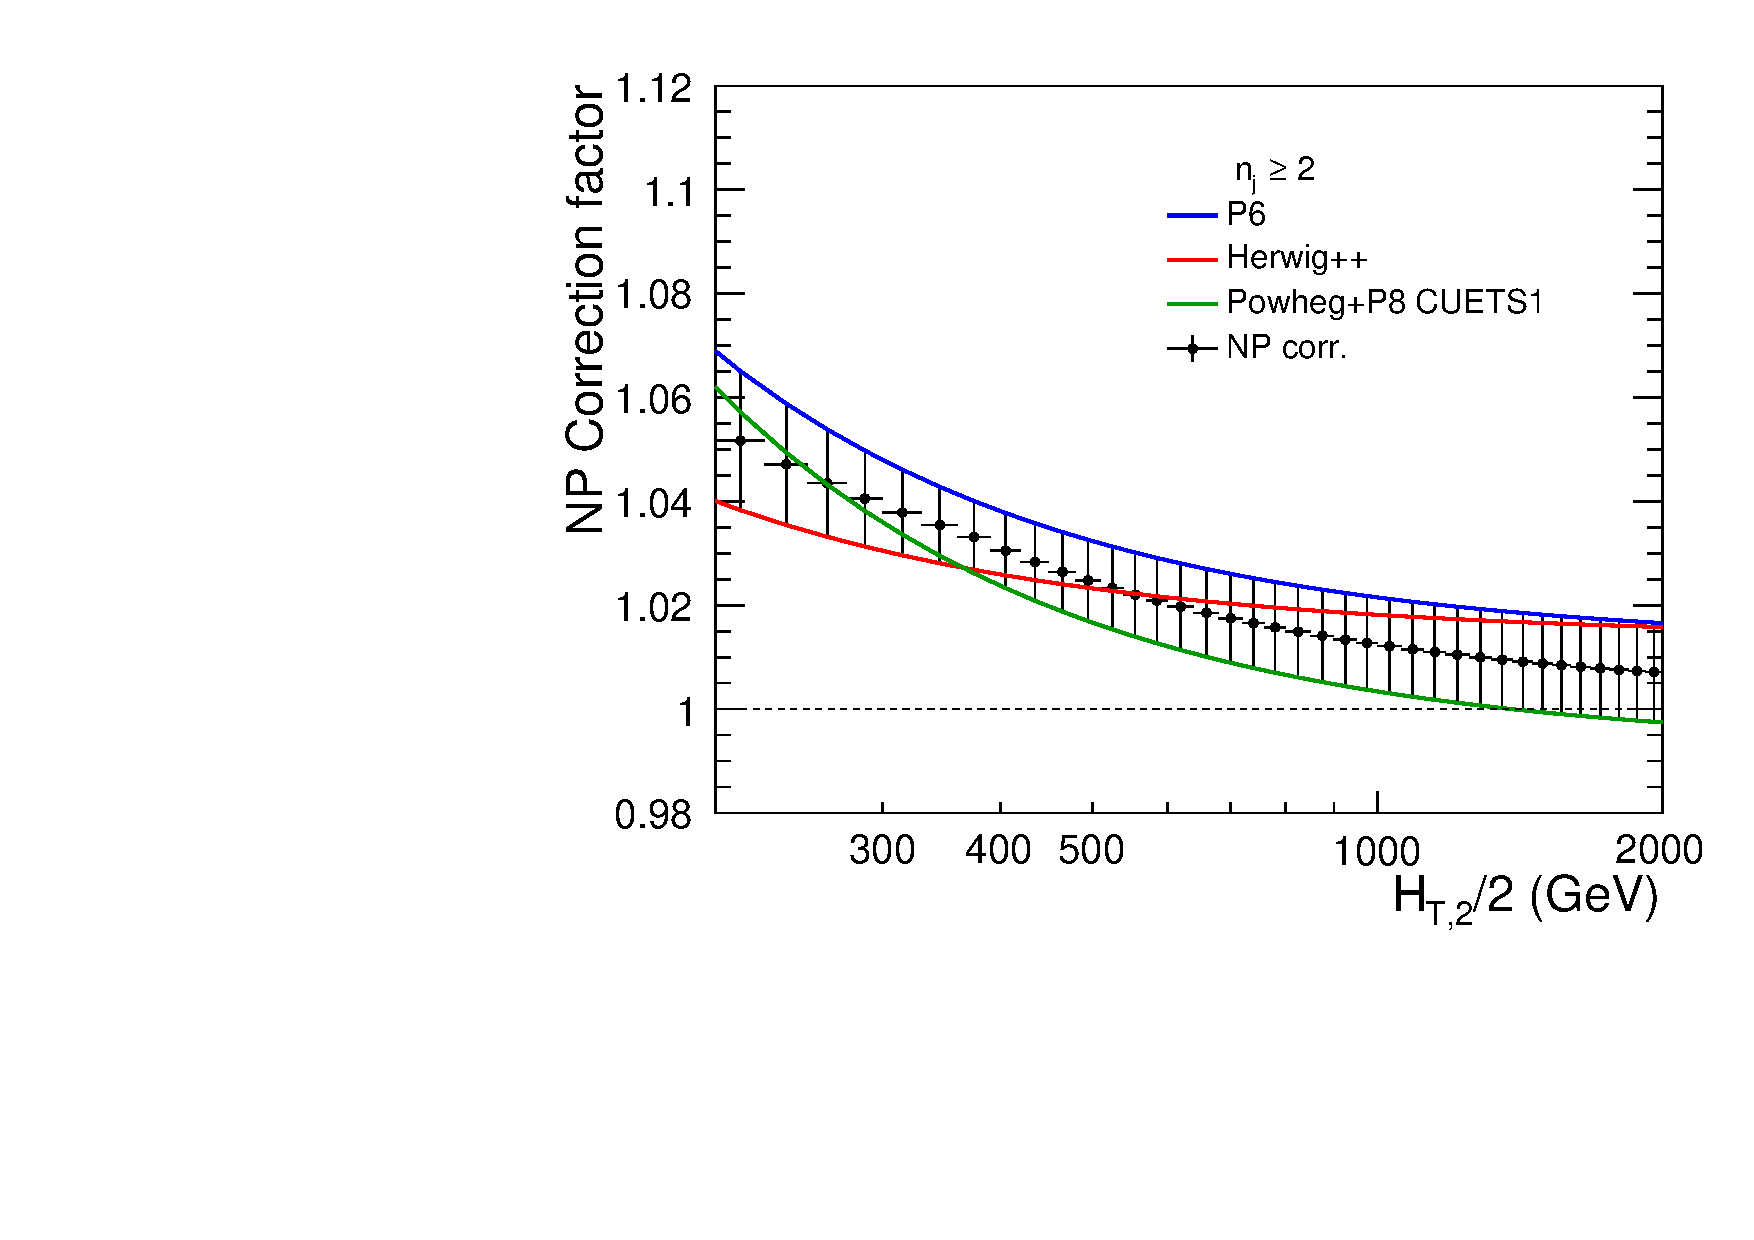
\includegraphics[width=0.5\textwidth]{Plots_PAS/Final_NP_Corr_2.pdf}\hftwo%
  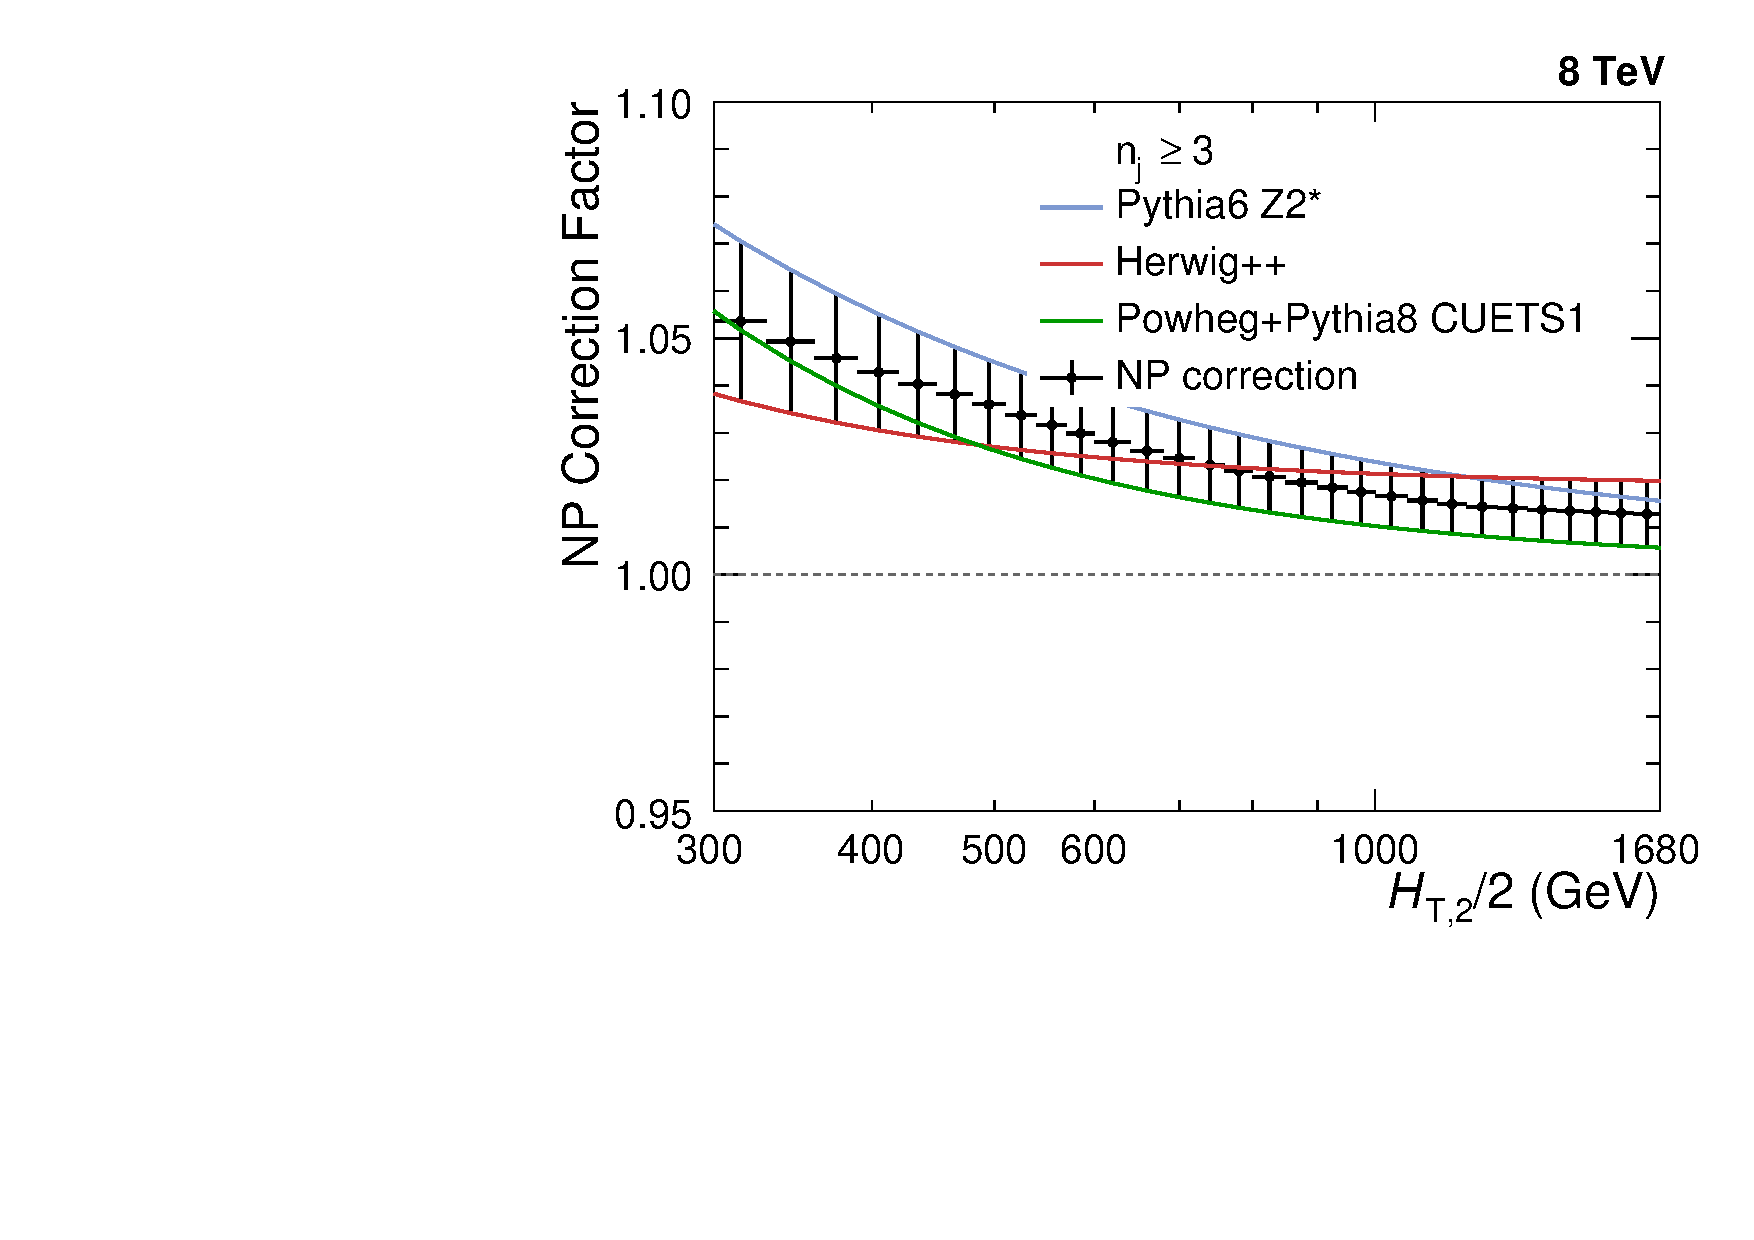
\includegraphics[width=0.5\textwidth]{Plots_PAS/Final_NP_Corr_3.pdf}\hftwo\\
  \hftwo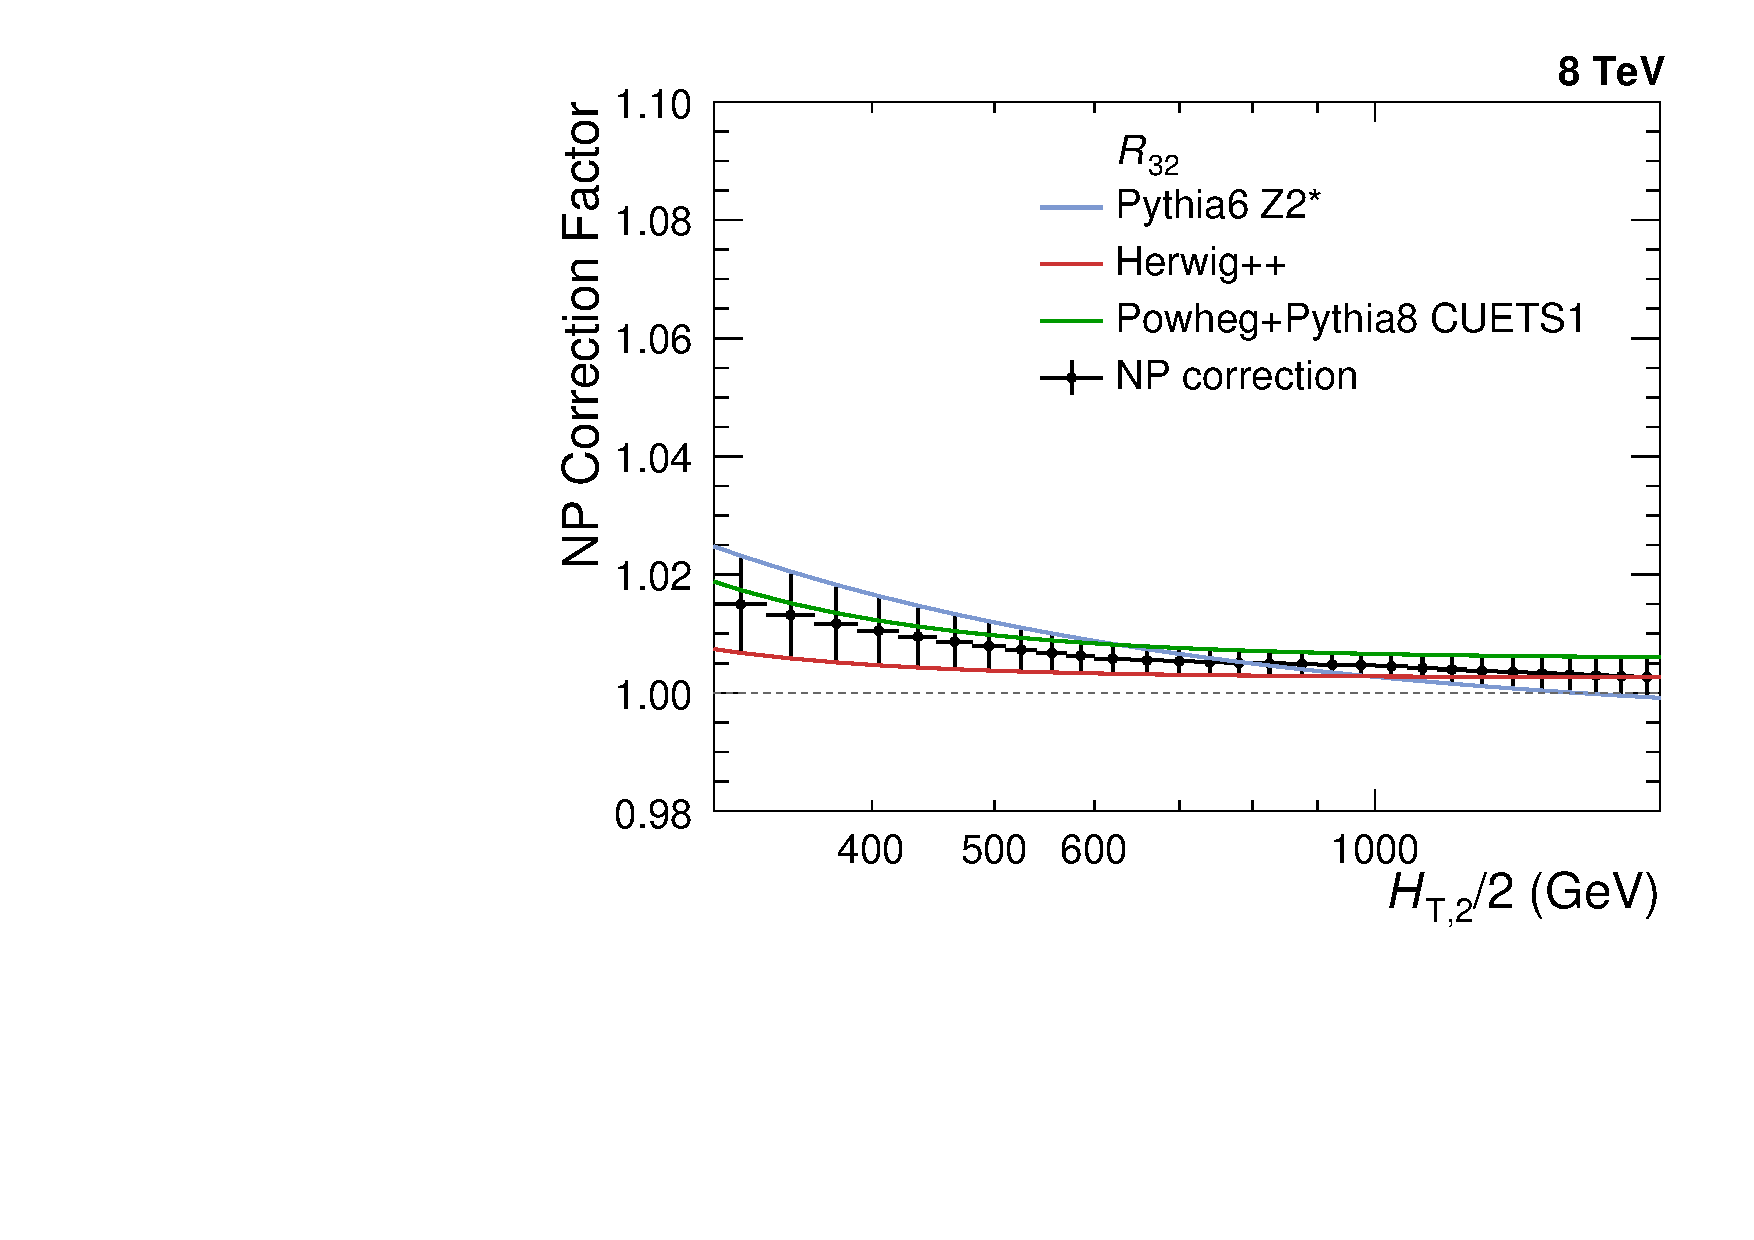
\includegraphics[width=0.5\textwidth]{Plots_PAS/Final_NP_Corr_Ratio_32.pdf}\hftwo
  \caption{Fits to the nonperturbative corrections obtained for
    inclusive 2-jet (top \cmsLeft) and 3-jet (top \cmsRight) event
    cross sections and their ratio \ratio (bottom) as a function of
    \httwo within $|y|<2.5$ for the three investigated MC event
    generators.}
  \label{fig:np_factors}
\end{figure}

The NP corrections are shown in Fig.~\ref{fig:np_factors} for the
inclusive 2-jet (top \cmsLeft) and 3-jet event cross sections (top
\cmsRight) as well for \ratio (bottom). They amount to $\approx$
4--5\% for inclusive 2-jet and 3-jet events and $\approx$ 1\% for
\ratio at \httwo $\approx$ 300\GeV and decrease for increasing
\httwo. The uncertainty assigned to the NP corrections is of the order
of 1--2\%. The non-perturbative effects are reduced in the cross
section ratio.

\begin{figure}[h]
  \hftwo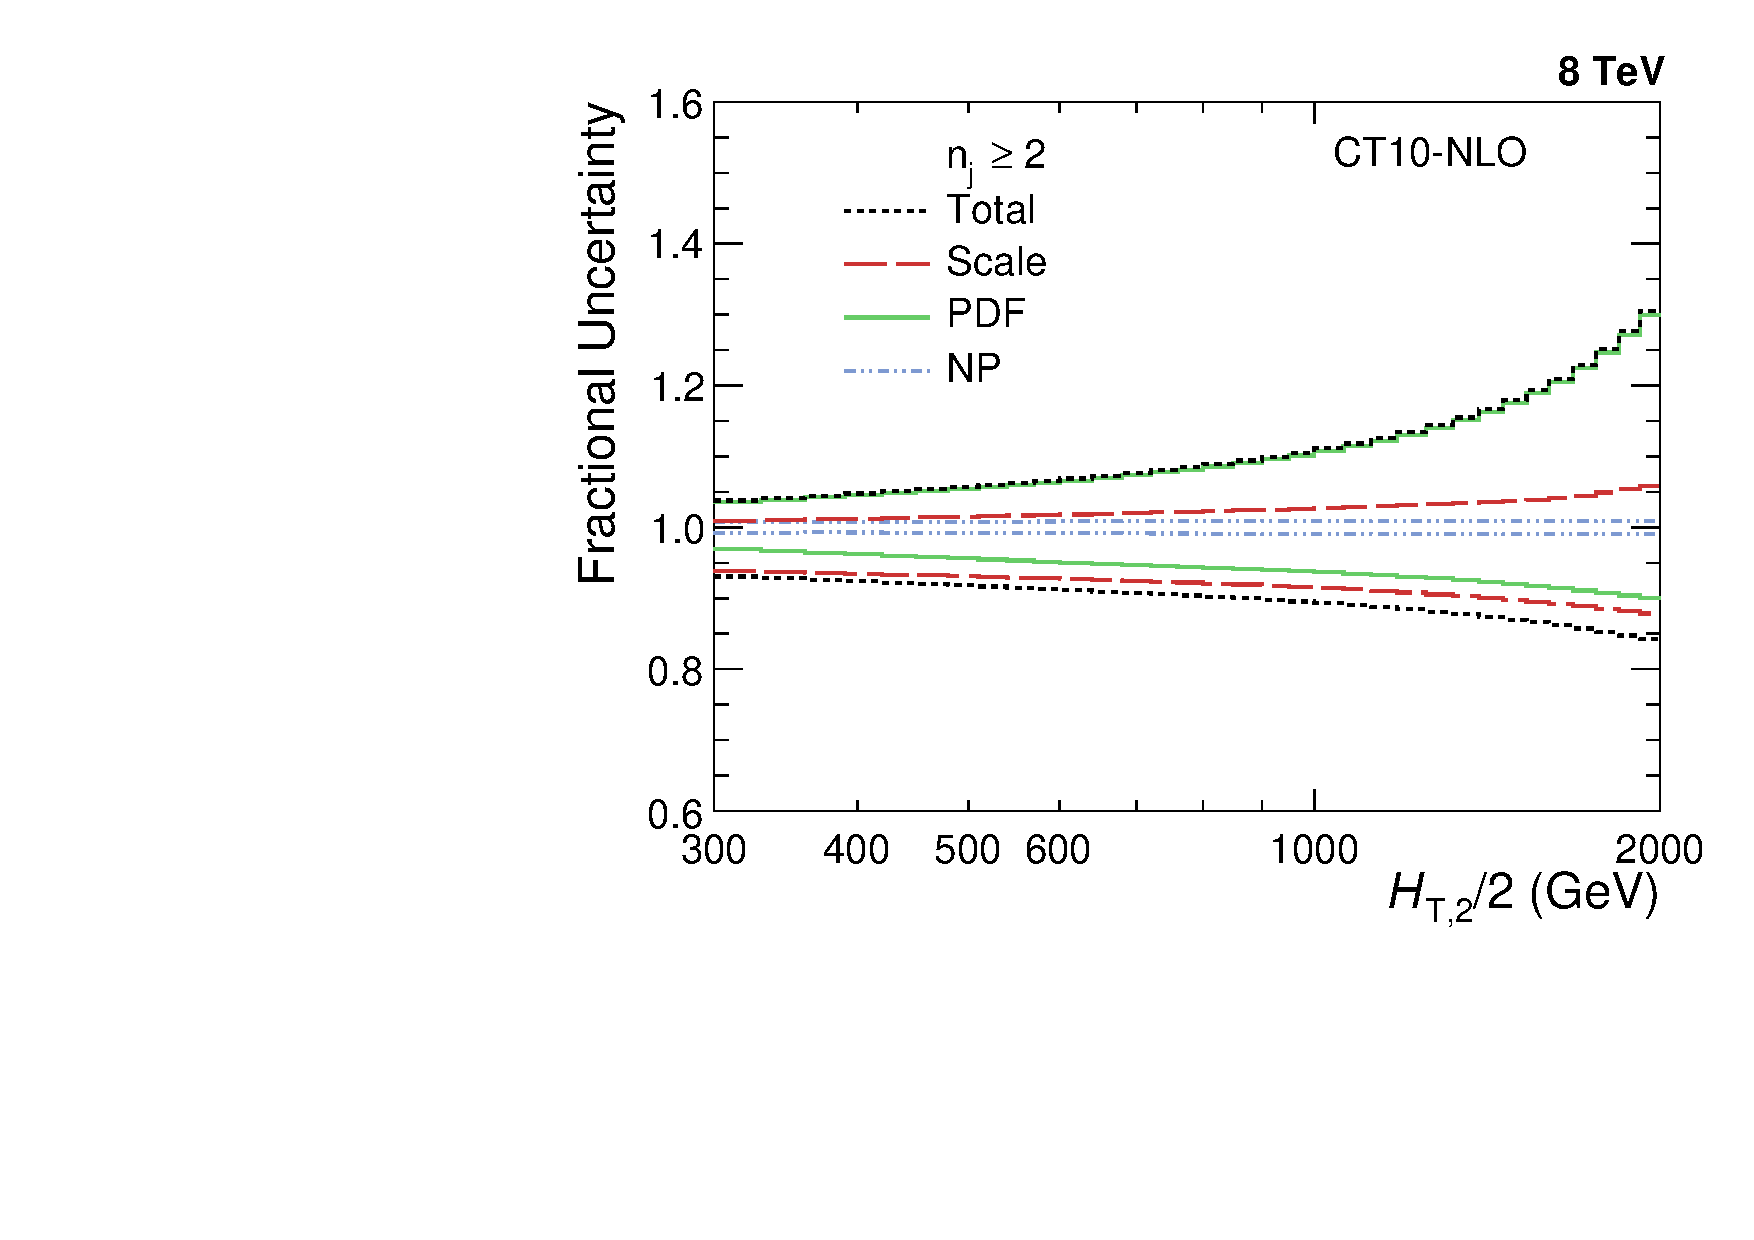
\includegraphics[width=0.5\textwidth]{Plots_PAS/Theory_Unc_2.pdf}\hftwo%
  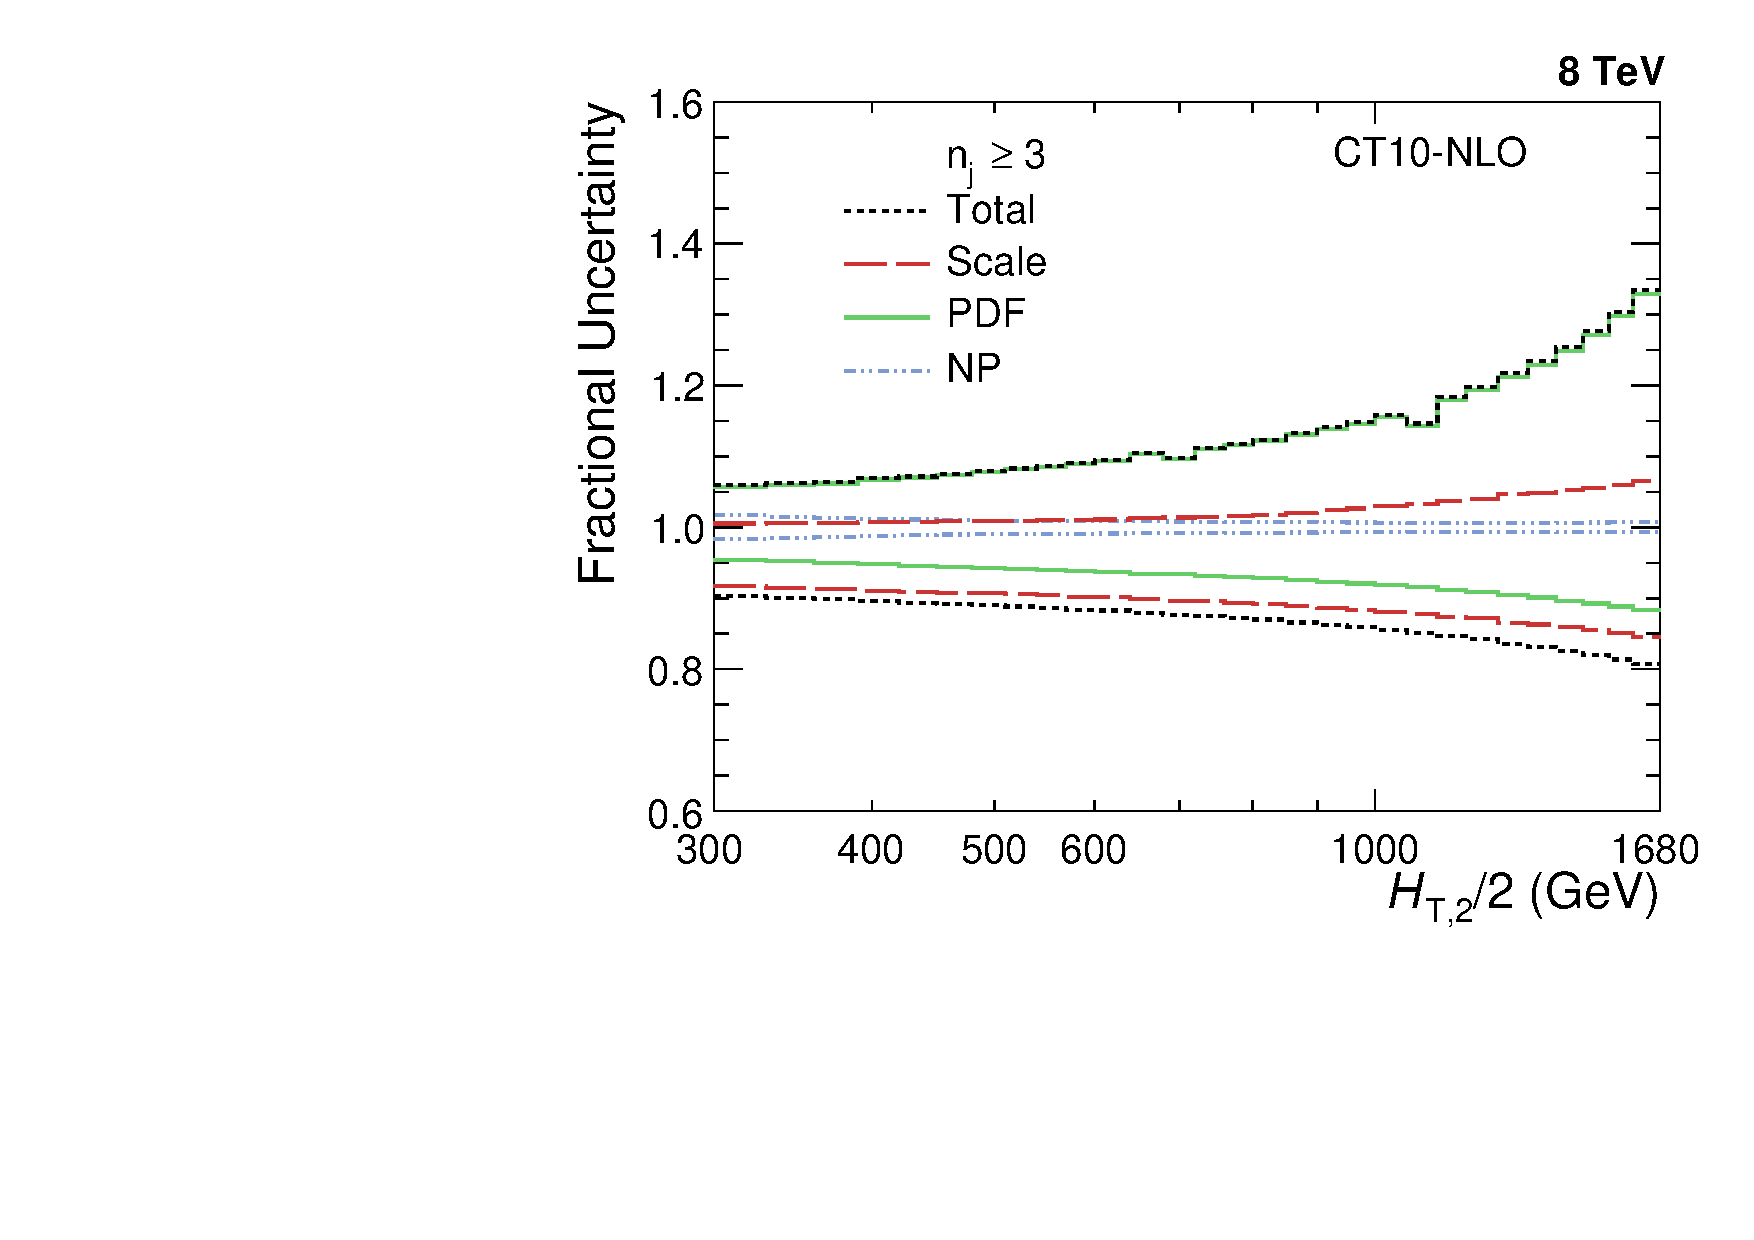
\includegraphics[width=0.5\textwidth]{Plots_PAS/Theory_Unc_3.pdf}\hftwo\\
  \hftwo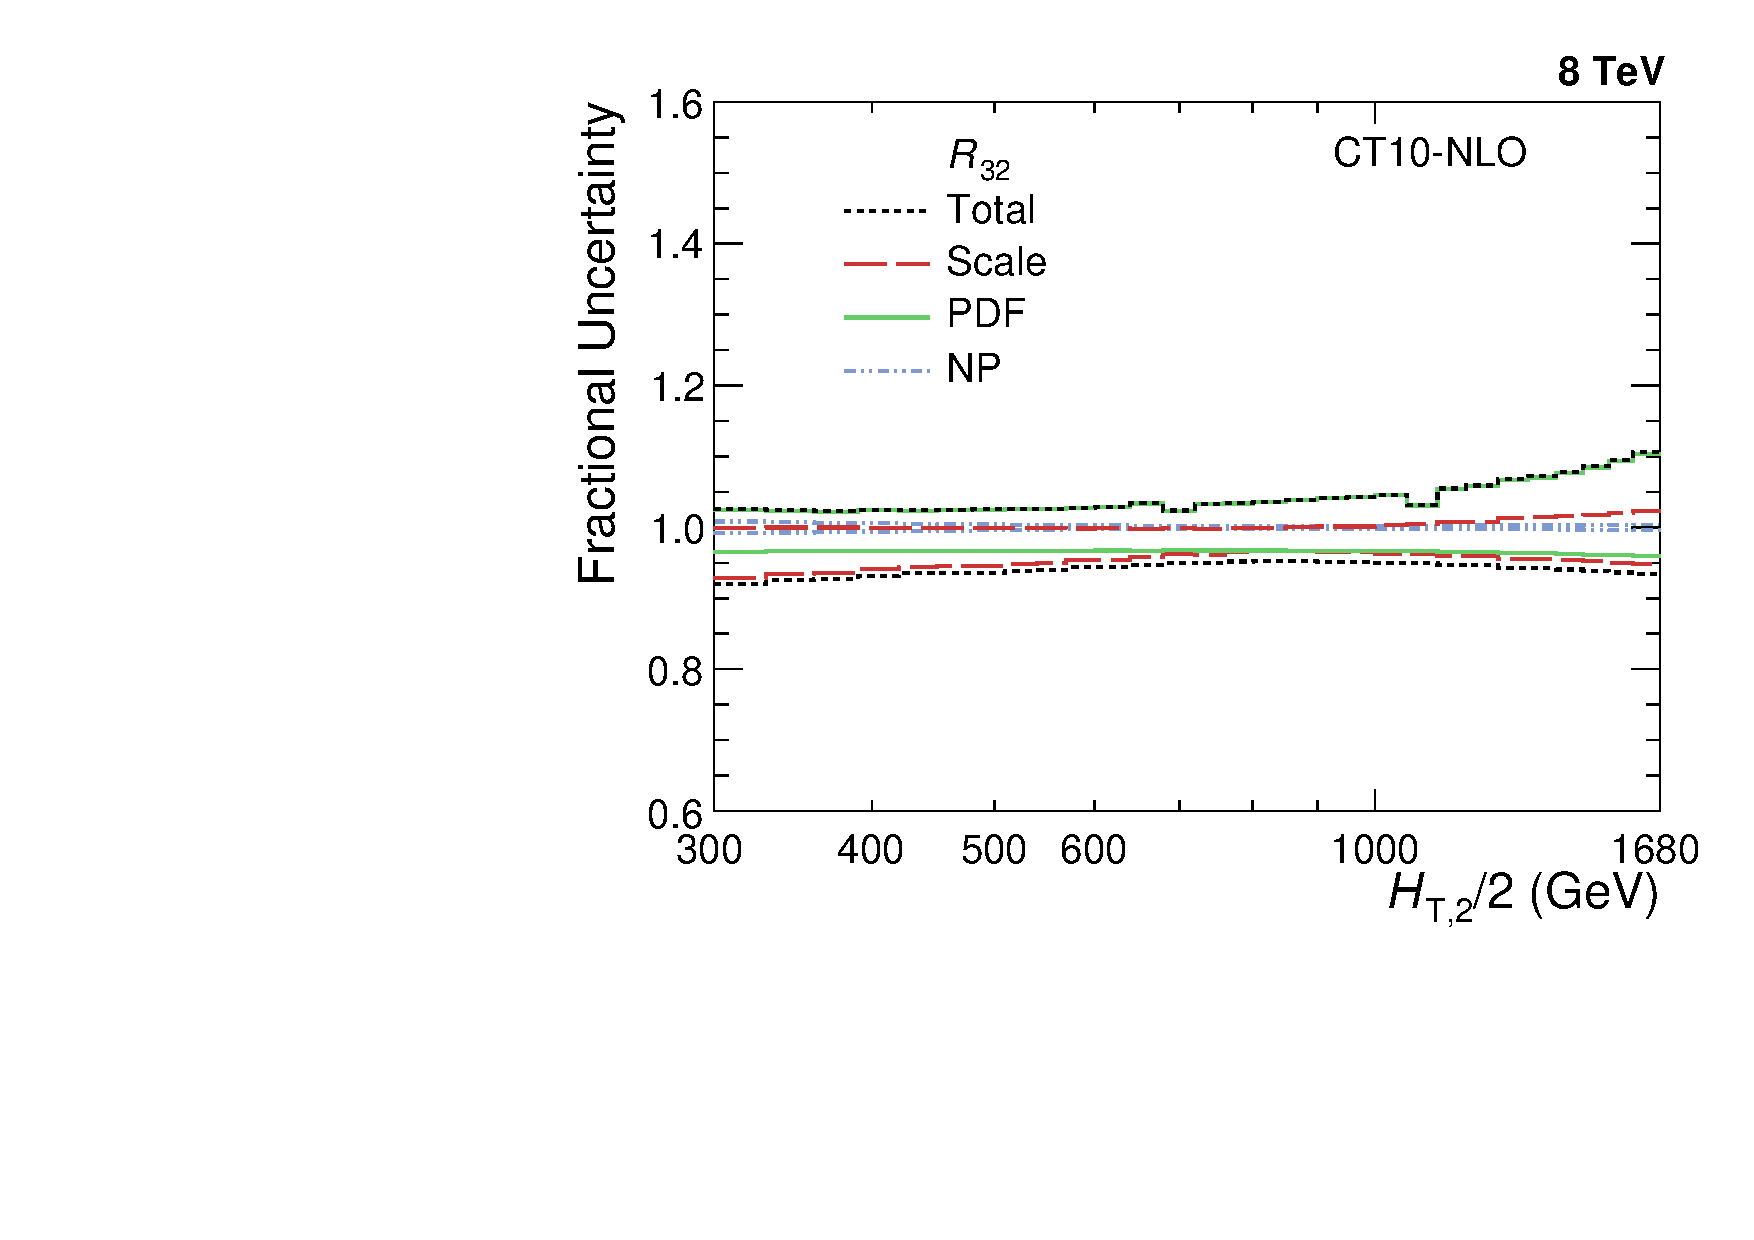
\includegraphics[width=0.5\textwidth]{Plots_PAS/Theory_Unc_Ratio_32.pdf}\hftwo
  \caption{Overview of theoretical uncertainties affecting the cross
    section prediction for inclusive 2-jet (top \cmsLeft) and 3-jet
    events (top \cmsRight) and their ratio \ratio (bottom), using the CT10 PDF set. The total uncertainty
    is calculated by adding in quadrature the individual sources of
    uncertainty. The statistical uncertainties of the NLO computations
    are too small to be visible and are not shown.}
  \label{fig:theory_unc}
\end{figure}

The total theoretical uncertainties are evaluated as the quadratic sum
of the scale, PDF, NP, and statistical
uncertainties. Figure~\ref{fig:theory_unc} presents an overview of the
theoretical uncertainties affecting the cross section prediction for
inclusive 2-jet (top \cmsLeft) and 3-jet events (top \cmsRight) and their ratio \ratio (bottom),
using the CT10 PDF set.
\end{comment}
